\subsection{Componentes} 
\begin{frame}{Input manager}
\begin{columns}
  \begin{column}{0.5\textwidth}
    \textbf{\underline{Blender}} (0 líneas)
    
	\begin{figure}
		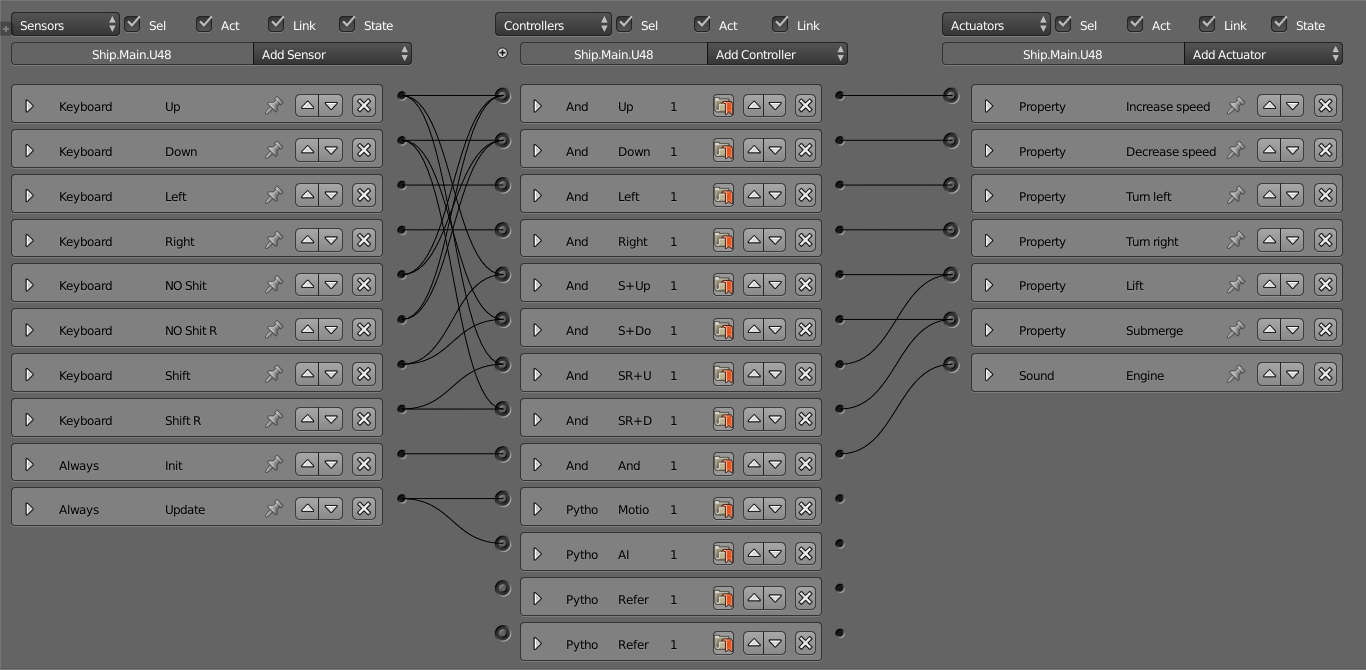
\includegraphics[scale=0.12]{blender_logic} 
	\end{figure}
  \end{column}

  \begin{column}{0.5\textwidth}
    \textbf{\underline{OGRE}} (\textcolor{red}{-1054-379} líneas)
    
    \vspace{0.4cm}
    Analizar las entradas por teclado y ratón en \CC $\,$ requiere generar una
    clase específica para ello haciendo uso de OIS (el estándar en OGRE hasta
    la versión 1.8).
    
    \begin{tikzpicture}[scale=0.8]
    	\node [whitebox] (Header file) at ($(-5,\vertspacing*1)$) {
    		\nodelabel{Header file}{\textit{204 líneas}}
    	};
    	\node [whitebox] (Source file) at ($(-5,\vertspacing*2)$) {
    		\nodelabel{Source file}{\textit{175 líneas}}
    	};
    \end{tikzpicture}    
  \end{column}
\end{columns}
\end{frame}

\begin{frame}{Input manager}
\begin{columns}
  \begin{column}{0.5\textwidth}
    \textbf{\underline{Blender}} (\textcolor{red}{-98} líneas)
    
    \vspace{0.5cm}
    \begin{tikzpicture}[scale=0.8]
    	\node [whitebox] (Camera inputs) at ($(-5,\vertspacing*1)$) {
    		\nodelabel{Camera inputs}{\textit{83 líneas}}
    	};
    	\node [whitebox] (Submarine inputs) at ($(-5,\vertspacing*2)$) {
    		\nodelabel{Submarine inputs}{\textit{15 líneas}}
    	};
    \end{tikzpicture}	
  \end{column}

  \begin{column}{0.5\textwidth}
    \textbf{\underline{OGRE}} (\textcolor{red}{-1054-379} líneas)
    
    \vspace{1.5cm}
    Sin implementar en OGRE
  \end{column}
\end{columns}
\end{frame}
